%
% main.tex -- Paper zum Thema komplexe Morlet Wavelets und CWT
%
% (c) 2019 Hochschule Rapperswil
%

\chapter{Komplexe Morlet Wavelets und CWT\label{chapter:thema}}
\lhead{Komplexe Wavelets und CWT}
\begin{refsection}
\chapterauthor{Roy Seitz}

Die schnelle Wavelettransformation (Fast Wavelet Transform, FWT) mit reellen Wavelets besitzt eine Vielzahl nützlicher Eigenschaften.
Je nach Anwendung besitzt sie jedoch auch zwei wesentliche Nachteile.

Erstens ist man sich aus der Fouriertheorie gewohnt, Phasen- und Amplitudeninformation getrennt betrachten zu können.
Diese Eigenschaft folg direkt aus der Wahl komplexer Basisfunktionen (oder Sinus und Cosinus als REal- und Imaginärteil der komplexen Schwingung) und ist mit reellen Wavelets folglich nicht möglich.

Als zweites sind die Frequenzen in der FWT nur in Zweierpotenzen der Abtastfrequenz berechnet, ähnlich der Fourier-Reihen, wo nur ganzzahlige Vielfache der Grundfrequenz berechnet werden.
Aus mathematischer Sicht ist das zwar ausreichend, für manche Anwendungen ist diese Auflösung jedoch zu grob.

Die Antworten hierzu fanden wir in Kapitel~\ref{chapter:cwt}, die kontinuierliche Wavelettransformation mit komplexen Wavelets (Continuous Wavelet Transform, CCWT).
Als erstes möchten wir folglich betrachten, wie wir mit komplexen Wavelets Amplituden- und Phasen-Information getrennt auswerten können und als zweites, wie wir geeignete Wavelets finden.

Als drittes möchten wir die CCWT effizient berechnen können.
Wir werden sehen, wie dies mittels Fourier-Transformation elegant erledigt werden kann.
Diese Berechnung liefert eine neue Interpretation der Wavelettransformation und führt zugleich zu einer Bedingung für nützliche Wavelets.

Abschliessend betrachten wir noch die Effekte der zyklischen Faltung, welche durch die FFT erzielt wird.
Dies führt zu -- möglicherweise störenden -- Randeffekten.
Deren Vermeidung ist durch padding des Sinal vermeidbar, was allerdings zusätzliche Rechenleistung erfordert.
Im letzten Teil dieses Kapitels betrachten wir folglich die Performance-Unterschiede, welche durch das PAdding entstehen.


%%%%%%%%%%%%%%%%%%%%%%%%%%%%%%%%%%%%%%%%%%%%%%%

\section{Das Morlet-Wavelet}
\rhead{Komplexe Wavelets}
Auch die reellen Fourierreihen haben das Problem, dass man Amplitude und Phase nicht separat betrachten kann, wenn man nur die Cosinus-Terme verwendet.
Dies liegt daran, dass Amplitude und Phase beim Cosinus gekoppelt sind,
\[
x = A\cos(\alpha) \quad\leftrightarrow\quad \alpha = \cos^{-1}\left(\frac{x}{A}\right).
\]
Erst durch die komplexe Schwingung 
\begin{align*}
	z(t) = Ce^{i\omega t} &= |C|e^{i\left(\omega t + \arg C\right)}
%	 &= |C|\left[\cos\left(\omega t + \arg C\right) + i \sin\left(\omega t + \arg C\right)\right]
\end{align*}
erhält man eine Basisfunktion, die mit
\[
	|z(t)| = |C| \quad \text{und}\quad
	\arg z = \arg \omega t + \arg C
\]
eine separate Betrachtung von Amplitude und Winkel erlaubt.
Diese Eigneschaft überträgt sich von den Basisfunktionen auf die Fouriertransformation.
Aufgrund der eulerschen Formel
\begin{equation}
	\cos(x) = \frac{e^{ix} + e^{-ix}}{2}\label{complex:euler}
\end{equation}
kann der Cosinus aus zwei komplexen Exponentialfunktionen mit inverser Frequenz dargestellt werden.
Besitzt ein Wavelet also negative Frequenz-Anteile, dann geht bei diesen Frequenzen die Eigenschaft der Separierbarkeit von Amplitude und Phase verloren.

\begin{figure}
	\centering
	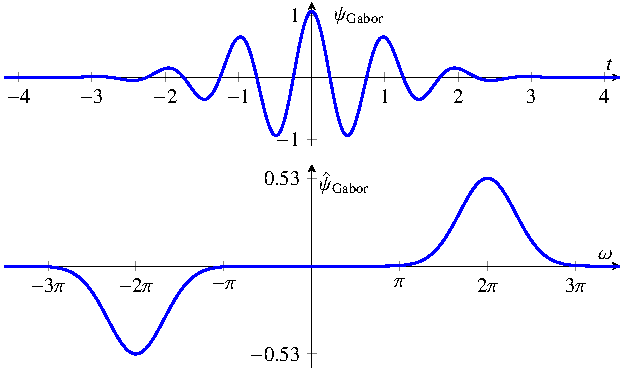
\includegraphics{papers/complex/images/gabor.pdf}
	\caption{Das Gabor-Wavelet für $\sigma = 2\pi$ \label{complex:gabor}}
\end{figure}

Ein geeignetes Wavelet benötigt folglich eine Fouriertransformierte, die bei negativen Frequenzen verschwindet.
Betrachten wir nun das Gabor-Wavelet
\[
	\psi = c_\sigma e^{-\frac{t^2}{2}}\left(\cos\left(\sigma t\right) - \kappa_\sigma\right),
\]
welches auch in Abbildung~\ref{complex:gabor} ersichtlich ist.
$c_\sigma$ und $\kappa_\sigma$ sind hierbei positive, reelle Konstanten, welche die Norm und die Zulässigkeitsbedingung~\eqref{cwt:zulaessig} korrigieren.
$\kappa_\sigma$ ist typischerweise sehr klein und wird oftmals einfach weggelassen.
Dieses Wavelet besitzt die dominante Frequenz $\sigma$ und ist durch die Gaus-Funktion in der Zeit lokalisiert.
Das Gabor-Wavelet eignet sich deshalb besonders gut, um einzelne Frequenzen in einem Signal zu finden.

Durch die Cosinus-Funktion besitzt das Gabor-Wavelet jedoch negative Frequenzen, wodurch eine isolierte Betrachtung von Amplitude und Phase unmöglich wird.
Dies möchten wir im Folgenden korrigieren.
Hierzu wechseln wir in den Fourierbereich.
Wir nutzen aus, dass die Fouriertransformierte einer Gaus-Kurve wieder eine Gauskurve ist,
\[
	\mathcal{F}\left\lbrace e^{-\alpha x^2} \right\rbrace 
	= \frac{1}{\sqrt{2\alpha}}e^{- \frac{\omega^2}{4\alpha}},
\]
und dass die Multiplikation im Zeitbereich zur Faltung im Frequenzbereich wird.
Zudem verwenden wir die Eulerformel~\eqref{complex:euler}.
Die Fouriertransformeirte des Gabor-Wavelet wird hierdurch zu
\[
 \hat{\psi} = 
 c_\sigma e^{- \frac{\omega^2}{2}} * \left(
  \frac{1}{2}\delta(\omega - \sigma) +
  \frac{1}{2}\delta(\omega + \sigma) + 
  \kappa_\sigma\delta(\omega)
  \right).
\]
Hierbei bezeichnet $\delta(\omega)$ die Dirac-Distribution.
Hieraus lässt sich der negative Anteil des Cosinus leicht entfernen.
Zudem verdoppeln wir den Anteil der positiven Frequenzen (der Grund hierfür erschliesst sich im nächsten Kapitel).
Wir erhalten
\[
	\hat{\psi}^\ast = 
	c_\sigma e^{- \frac{\omega^2}{2}} * \left(
	\delta(\omega - \sigma) +
	\kappa_\sigma\delta(\omega)
	\right),
\]
und durch Rücktransformation in den Zeitbereich
\[
	\psi^\ast = 
	c_\sigma e^{- \frac{t^2}{2}} \cdot \left(
	e^{i\sigma t} +
	\kappa_\sigma
	\right).
\]
Dies ist ein alter Bekannter, das Morlet-Wavelet aus Gleichung~\eqref{cwt:morlet}.
Abbildung~\ref{complex:morlet} zeigt den Real- und Imaginärteil, so wie die Envelope des Morlet-Wavelets.
Die Unabhängigkeit der Amplitude und der Phase 
Die Envelope entspricht hierbei gerade dem Absolutwert.
Das Morlet-Wavelet eignet sich also besonder gut, um bestimmte Frequenzen in einem Signal zu lokalisieren.
Im nächsten Kapitel werden wir sehen, dass man aus jedem, reellen Wavelet eines konstruieren kann, welches eine separate Betrachtung von Amplitude und Phase ermöglicht.

\begin{figure}
	\centering
	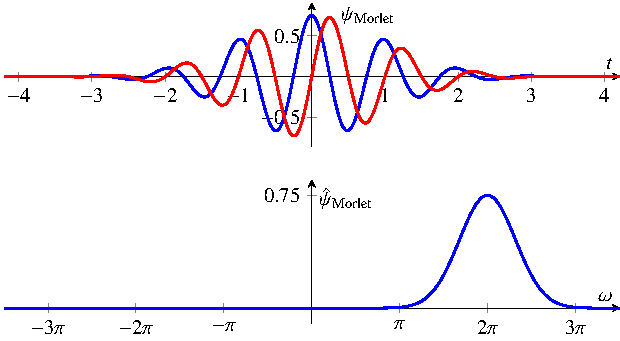
\includegraphics{papers/complex/images/morlet.pdf}
	\caption{Real- (blau) und Imaginärteil (rot) des Morlet-Wavelet für $\sigma = 2\pi$ \label{complex:morlet}}
\end{figure}


\section{Analytische Wavelets und Hilbert-Transformation}
\subsection{Analytische Signals}
\rhead{Analytische Signale}
Im ersten Kapitel haben wir aus dem reellen Gabor-Wavelet und dem Wunsch nach Separation von Amplitude und Phase das komplexe Morlet-Wavelet gefunden.
Hierzu haben wir die negativen Frequenzen aus dem Spektrum des Wavelets entfernt.
Dieses Verfahren lässt isch mit der Hilbert-Transformation
\[
	\mathcal{H}f(t) =
	\frac{1}{\pi}\int_{-\infty}^{\infty}\frac{f(x)}{t-x} dx
\]
elegant verallgemeinern.
Hierzu benötigen wir den Begriff des analytischen Signals.
\begin{definition}
	Sei $f(t) \in \mathbb{R}$ ein reelles Zeitsignal, dann heisst
	\begin{align*}
		f^\ast(t) 
		&= f(t) + i\,\mathcal{H}f(t)
	\end{align*}
	das zu $f(t)$ \emph{analytische Signal}\footnote{Der Begriff `analytisch' ist in diesem Kapitel immer im Sinne dieser Definition aus der Signaltheorie zu verstehen.
	Er ist nicht zu verwechseln mit der Eigenschaft analytischer Funktionen in der Analysis.
%	Die Analysis kennt den Begriff der analytischen Funktion. 
%	Diese Eigenschaft ist in der komplexen Analysis jedoch äquivalent zur Holomorphie.
%	Wo benötigt wird folglich von holomorphen Funktionen gesprochen, um Verwechslungen zu vermeiden.
	}.
\end{definition}

\begin{satz}
	Die Fourier-Transformierte eines analytischen Signals verschwindet für alle negativen Frequenzen.
	Es gilt
	\[
		\hat{f}^\ast_{a,b}(\omega) = \left\lbrace\begin{matrix*}[r]	
			2\hat{f}_{a,b} & 0 \le \omega \\ 0 & \text{sonst}\end{matrix*} \right..
	\]
\end{satz}

\begin{proof}[Beweis]
	Die Hilbert-Transformation besitzt die Form eines Faltungs-Integrals.
	Es gilt
	\begin{align*}
		\mathcal{H} f(t) &= f(t) * \frac{1}{\pi t}.
	\end{align*}
	Diese Faltung wird im Frequenzbereich zur Multiplikation.
	Mit der Signumsfunktion $\sgn(\omega)$ und der Identität
	\begin{align*}
		\mathcal{F} \left\lbrace t^{-1}\right\rbrace  &= -i\pi\sgn(\omega)
	\end{align*}
	wird die Hilberttransformation im Frequenzbereich zu
	\begin{align*}
		\mathcal{F}\left\lbrace \mathcal{H}f(t)\right\rbrace 
		&= -i\sgn(\omega) \hat{f}.
	\end{align*}
	Für die Fourier-Transformierte von $f^\ast_{a,b}$ gilt folglich 
	\begin{align*}
		\hat{f}^\ast_{a,b} 
		&= \hat{f}_{a,b} - i^2\sgn(\omega)\hat{f}_{a,b}\\
		&=\left\lbrace\begin{matrix}
			2\hat{f}_{a,b} & \omega > 0\\
			0 & \omega \le 0
		\end{matrix} \right.
	\end{align*}
\end{proof}

Mittels Hilbert-Transformation kann man also aus jedem beliebigen, reellen Zeitsignal ein analytisches Signal konstruieren.
Spektral ist dies gleichbedeutend damit, die negativen Frequenzen zu entfernen und die positiven zu verdoppeln, wie wir das im ersten Kapitel auf dem Weg vom Gabor- zum Morlet-Wavelet auch getan haben.
Tatsächlich ist das Morlet-Wavelet das zum Gabor-Wavelet analytische Wavelet.
Die Norm erhöht sich hierbei jedoch um den Faktor $\sqrt{2}$.
Beim Gabor- und Morlet-Wavelet versteckt sich dieser Faktor im $c_\sigma$.

\subsection{Analytische Wavelets und deren Norm}
\rhead{Analytische WAvelets}

Die Norm eines Wavelets muss $1$ sein.
Folglich muss die Norm und jene, des zum Original-Wavelet analytischen Wavelets gleich sein.
Bei analytischen Signalen ist dies jedoch nicht gegeben.
Dies führt zur
\begin{definition}
	Sei $\psi$ ein beliebiges, reelles Wavelet. Dann ist
	\[
	\psi^\ast = \frac{1}{\sqrt{2}}\left(\psi + i\,\mathcal{H}\psi\right) 
	\]
	das zu $\psi$ \emph{analytische Wavelet}.
\end{definition}

Für die Norm eines analytischen Wavelets gilt
\begin{satz}
	\label{complex:norm}
	Die Norm eines analytischen Wavelets ist gleich der Norm des Original-Wavelets.
	\[\left\|\psi\right\| = \left\|\psi^\ast\right\|\].
\end{satz}

\begin{proof}
	Wir rechnen nach:
	\begin{align*}
		\left\|\psi\right\| = \left\|\hat{\psi}\right\|
		&= \int_{-\infty}^{\infty}\left|\hat{\psi}(\omega)\right|^2 d\omega \\
		&= \int_{-\infty}^{0}\left|\hat{\psi}(\omega)\right|^2 d\omega +  \int_{0}^{\infty}\left|\hat{\psi}(\omega)\right|^2 d\omega \\
		&=  2\int_{0}^{\infty}\left|\hat{\psi}(\omega)\right|^2 d\omega \\
		&=  \int_{0}^{\infty}\left|\frac{2}{\sqrt{2}}\hat{\psi}(\omega)\right|^2 d\omega \\
		&=  \int_{-\infty}^{\infty}\left|\hat{\psi}^\ast(\omega)\right|^2 d\omega 
		= \left\|\hat{\psi}^\ast\right\| = \left\|\psi^\ast\right\|.
	\end{align*}
	Hierbei haben wir zu begin und am Ende die Placherel-Formel verwendet.
	In Zeile drei nutzten wir die hermitesche Symmetrie der Fourier-Transformierten eines reellen Wavelets, nach welcher
	\[\left|\hat{f}(\omega)\right| = \left|\hat{f}(-\omega)\right|\]
	gilt.
	Somit ist Satz~\ref{complex:norm} bewiesen.
\end{proof}

\subsection{Analytisches Haar-Wavelet}
\rhead{Analytisches Haar-WAvelet
}
Betrachten wir zum Abschluss noch beispielhaft das Haar-Wavelet
\[
	\psi_{\text{Haar}} = \left\lbrace\begin{matrix*}[r]
		1 & 0 \le t < \frac{1}{2} \\
		-1 & \frac{1}{2} \le t < 1 \\
		0 & \text{sonst}
	\end{matrix*} \right..
\]
Die Hilbert-Transformierte des Haar-Wavelets berechnet sich zu
\begin{align*}
	\mathcal{H} \psi_{\text{Haar}}
	&= \frac{1}{\pi} \int_{-\infty}^{\infty} \frac{\psi_{\text{Haar}}(x)}{t-x} dx\\
	&= \frac{1}{\pi}\left( \int_{0}^{0.5} \frac{1}{t-x}dx + \int_{0.5}^{1} \frac{-1}{t-x}dx \right)\\
	&= \frac{1}{\pi} \left( -\left[\log \left|t-x\right| \right]_0^{0.5} + \left[\log\left|t-x\right| \right]_{0.5}^{1} \right)\\
	&= \frac{1}{\pi} \left( -\log\left|t-0.5\right| + \log\left|t\right| + \log\left|t-1\right| - \log\left|t-0.5\right|\right)\\
	&= \frac{1}{\pi} \log\left|\frac{t(t-1)}{(t-0.5)^2}\right|
\end{align*}

Die analytische Form des Haar-Wavelet ist also
\[
 \psi^\ast_{\text{Haar}} = \frac{1}{\sqrt{2}}\left(\psi_{\text{Haar}} + \frac{i}{\pi} \log\left|\frac{t(t-1)}{2(t-0.5)^2}\right|\right)
\]
Diese Funktion ist in Abbildung~\ref{complex:haar} dargestellt.
Das analytische Haar-Wavelet hat offensichtlich keinen kompakten Träger mehr.
Zudem ist auch die Norm nicht mehr dieselbe.

\begin{figure}
	\centering
	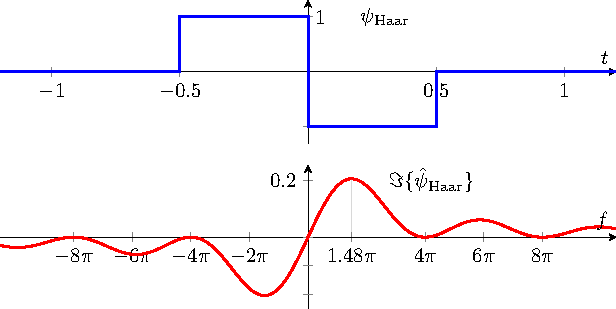
\includegraphics{papers/complex/images/haar.pdf}
	\caption{Das Haar-Wavelet (blau) und seine Hilbert-Transformierte (rot)
		\label{complex:haar}}
\end{figure}

%% An dieser Stelle fehlt noch die Betrachtung der Norm.
%% 1. Via Plancherel ||\psi^\ast|| = || \hat{\psi}^\ast ||
%% 2. Für reelle Psi gilt || \hat{\psi} || = je 1/2 || \hat{\psi} || von \omega > 0 und \omega < 0
%% 3. Für \omega < 0 alles weg, dafür doppelt^2 von \omega > 0 -> norm verdoppelt
%% 4. Damit ||\psi|| = 1/\sqrt{2} || \psi^\ast||
%% Neuer Normierungsfaktor, einfügen in der Definition des analytischen Signals und im Beweis hinzufügen. (im Gabor / Morlet-Wavelet im c_\sigma versteckt ohne zu erwähnen) 

\section{Schnelle Berechnung der kontinuierlichen komplexen Wavelettransformation}
\rhead{CCWT}

%% Wavelet-TraFo als Faltung zwischen Signal und Wavelet
%% Morlet-Wavelet in Frequenzbereich geschlossen berechenbar
%%  -> Faltungs-Matrix mit verschieden skalierten Morlet-Wavelets in den Spalten
%%   - Matrix-Multiplikation mit Signal
%%   - ifft über die Spalten

\section{Zyklische Faltung, Signal-Padding und Performanz}
\rhead{Zyklische Faltung}
%% Effekt der zyklischen Faltung
%% Lösen durch padden des Signals
%%  - zero padding
%%  - padden durch spiegeln des Signals
%% Performanz-Vergleich anhand Matlab-Skript

\section{Schlussfolgerung}
\rhead{Schlussfolgerung}
%% Jedes Wavelet kann in ein analytisches transformiert werden
%% Die Wavelets aus der FWT sind allerdings für die CWT ungeeignet, 
%% da sie nich in geschlossener Form im Frequenzbereich berechnet werden können
%% (Aufstellen der Faltungs-Matrix)
%% Allerdings ist das Morlet-WAvelet auch zu bevorzugen, da es die optimale 
%% Schärfe zwischen Frequenz- und Zeitauflösung beitet (Gaus\ldots)

\printbibliography[heading=subbibliography]
\end{refsection}
